% Template for PLoS
% Version 3.5 March 2018
%
% % % % % % % % % % % % % % % % % % % % % %
%
% -- IMPORTANT NOTE
%
% This template contains comments intended 
% to minimize problems and delays during our production 
% process. Please follow the template instructions
% whenever possible.
%
% % % % % % % % % % % % % % % % % % % % % % % 
%
% Once your paper is accepted for publication, 
% PLEASE REMOVE ALL TRACKED CHANGES in this file 
% and leave only the final text of your manuscript. 
% PLOS recommends the use of latexdiff to track changes during review, as this will help to maintain a clean tex file.
% Visit https://www.ctan.org/pkg/latexdiff?lang=en for info or contact us at latex@plos.org.
%
%
% There are no restrictions on package use within the LaTeX files except that 
% no packages listed in the template may be deleted.
%
% Please do not include colors or graphics in the text.
%
% The manuscript LaTeX source should be contained within a single file (do not use \input, \externaldocument, or similar commands).
%
% % % % % % % % % % % % % % % % % % % % % % %
%
% -- FIGURES AND TABLES
%
% Please include tables/figure captions directly after the paragraph where they are first cited in the text.
%
% DO NOT INCLUDE GRAPHICS IN YOUR MANUSCRIPT
% - Figures should be uploaded separately from your manuscript file. 
% - Figures generated using LaTeX should be extracted and removed from the PDF before submission. 
% - Figures containing multiple panels/subfigures must be combined into one image file before submission.
% For figure citations, please use "Fig" instead of "Figure".
% See http://journals.plos.org/plosone/s/figures for PLOS figure guidelines.
%
% Tables should be cell-based and may not contain:
% - spacing/line breaks within cells to alter layout or alignment
% - do not nest tabular environments (no tabular environments within tabular environments)
% - no graphics or colored text (cell background color/shading OK)
% See http://journals.plos.org/plosone/s/tables for table guidelines.
%
% For tables that exceed the width of the text column, use the adjustwidth environment as illustrated in the example table in text below.
%
% % % % % % % % % % % % % % % % % % % % % % % %
%
% -- EQUATIONS, MATH SYMBOLS, SUBSCRIPTS, AND SUPERSCRIPTS
%
% IMPORTANT
% Below are a few tips to help format your equations and other special characters according to our specifications. For more tips to help reduce the possibility of formatting errors during conversion, please see our LaTeX guidelines at http://journals.plos.org/plosone/s/latex
%
% For inline equations, please be sure to include all portions of an equation in the math environment.  For example, x$^2$ is incorrect; this should be formatted as $x^2$ (or $\mathrm{x}^2$ if the romanized font is desired).
%
% Do not include text that is not math in the math environment. For example, CO2 should be written as CO\textsubscript{2} instead of CO$_2$.
%
% Please add line breaks to long display equations when possible in order to fit size of the column. 
%
% For inline equations, please do not include punctuation (commas, etc) within the math environment unless this is part of the equation.
%
% When adding superscript or subscripts outside of brackets/braces, please group using {}.  For example, change "[U(D,E,\gamma)]^2" to "{[U(D,E,\gamma)]}^2". 
%
% Do not use \cal for caligraphic font.  Instead, use \mathcal{}
%
% % % % % % % % % % % % % % % % % % % % % % % % 
%
% Please contact latex@plos.org with any questions.
%
% % % % % % % % % % % % % % % % % % % % % % % %

\documentclass[10pt,letterpaper]{article}
\usepackage[top=0.85in,left=2.75in,footskip=0.75in]{geometry}

% amsmath and amssymb packages, useful for mathematical formulas and symbols
\usepackage{amsmath,amssymb}

% Use adjustwidth environment to exceed column width (see example table in text)
\usepackage{changepage}

% Use Unicode characters when possible
\usepackage[utf8x]{inputenc}

% textcomp package and marvosym package for additional characters
\usepackage{textcomp,marvosym}

% cite package, to clean up citations in the main text. Do not remove.
\usepackage{cite}

% Use nameref to cite supporting information files (see Supporting Information section for more info)
\usepackage{nameref,hyperref}

% line numbers
\usepackage[right]{lineno}

% ligatures disabled
\usepackage{microtype}
\DisableLigatures[f]{encoding = *, family = * }

% color can be used to apply background shading to table cells only
\usepackage[table]{xcolor}

% array package and thick rules for tables
\usepackage{array}

% multirow for multiple row tables. 
\usepackage{multirow}

% create "+" rule type for thick vertical lines
\newcolumntype{+}{!{\vrule width 2pt}}

% create \thickcline for thick horizontal lines of variable length
\newlength\savedwidth
\newcommand\thickcline[1]{%
  \noalign{\global\savedwidth\arrayrulewidth\global\arrayrulewidth 2pt}%
  \cline{#1}%
  \noalign{\vskip\arrayrulewidth}%
  \noalign{\global\arrayrulewidth\savedwidth}%
}

% \thickhline command for thick horizontal lines that span the table
\newcommand\thickhline{\noalign{\global\savedwidth\arrayrulewidth\global\arrayrulewidth 2pt}%
\hline
\noalign{\global\arrayrulewidth\savedwidth}}


% Remove comment for double spacing
%\usepackage{setspace} 
%\doublespacing

% Text layout
\raggedright
\setlength{\parindent}{0.5cm}
\textwidth 5.25in 
\textheight 8.75in

% Bold the 'Figure #' in the caption and separate it from the title/caption with a period
% Captions will be left justified
\usepackage[aboveskip=1pt,labelfont=bf,labelsep=period,justification=raggedright,singlelinecheck=off]{caption}
\renewcommand{\figurename}{Fig}

% Use the PLoS provided BiBTeX style
\bibliographystyle{plos2015}

% Remove brackets from numbering in List of References
\makeatletter
\renewcommand{\@biblabel}[1]{\quad#1.}
\makeatother



% Header and Footer with logo
\usepackage{lastpage,fancyhdr,graphicx}
\usepackage{epstopdf}
%\pagestyle{myheadings}
\pagestyle{fancy}
\fancyhf{}
%\setlength{\headheight}{27.023pt}
%\lhead{\includegraphics[width=2.0in]{PLOS-submission.eps}}
\rfoot{\thepage/\pageref{LastPage}}
\renewcommand{\headrulewidth}{0pt}
\renewcommand{\footrule}{\hrule height 2pt \vspace{2mm}}
\fancyheadoffset[L]{2.25in}
\fancyfootoffset[L]{2.25in}
\lfoot{\today}

%% Include all macros below

\newcommand{\lorem}{{\bf LOREM}}
\newcommand{\ipsum}{{\bf IPSUM}}

%% END MACROS SECTION


\begin{document}
\vspace*{0.2in}

% Title must be 250 characters or less.
\begin{flushleft}
{\Large
\textbf\newline{Joint modelling of aggregated incidence data and point prevalence surveys for malaria mapping} % Please use "sentence case" for title and headings (capitalize only the first word in a title (or heading), the first word in a subtitle (or subheading), and any proper nouns).
}
\newline
% Insert author names, affiliations and corresponding author email (do not include titles, positions, or degrees).
\\
Tim C.D. Lucas*\textsuperscript{1}, Anita Nandi\textsuperscript{1}, Michele Nguyen\textsuperscript{1}, Susan Rumisha \textsuperscript{1}, Ewan Cameron\textsuperscript{1}, Pete Gething\textsuperscript{1} and Dan Weiss\textsuperscript{1},
\\
\bigskip
\textbf{1} BDI, Oxford
\\
\bigskip

% Insert additional author notes using the symbols described below. Insert symbol callouts after author names as necessary.
% 
% Remove or comment out the author notes below if they aren't used.
%

% Current address notes



% Use the asterisk to denote corresponding authorship and provide email address in note below.
* timcdlucas@gmail.com

\end{flushleft}
% Please keep the abstract below 300 words
\section*{Abstract}
malaria is bad but decreasing
moving to strategy of elimination country by country
elimination requires maps of low prevalence areas
but maps in low prevalence areas are difficult
sometimes little data
traditional prevalence mapping won't work
we need new sources of data.



% Please keep the Author Summary between 150 and 200 words
% Use first person. PLOS ONE authors please skip this step. 
% Author Summary not valid for PLOS ONE submissions.   
\section*{Author summary}
malaria is bad but decreasing
moving to strategy of elimination country by country
elimination requires maps of low prevalence areas
but maps in low prevalence areas are difficult
sometimes little data
traditional prevalence mapping won't work
we need new sources of data.


\linenumbers

% Use "Eq" instead of "Equation" for equation citations.
%%%%%%%%%%%%%%%%%%%%%%%%%%%%%%%%%%%%%%%%%%%%%%%%%%%%%%%%%%%%%%%%%%%%%%%%%%%%%%%%%%%%%%%%%%%%%%%%%%%%%
\section*{Introduction}
%%%%%%%%%%%%%%%%%%%%%%%%%%%%%%%%%%%%%%%%%%%%%%%%%%%%%%%%%%%%%%%%%%%%%%%%%%%%%%%%%%%%%%%%%%%%%%%%%%%%%

Global malaria incidence has decreased dramatically over the last 20 years \cite{abajobir2017global, bhatt2015effect}.
This decrease has been accompanied by a strategic shift towards aiming for elimination in low incidence countries \cite{world2016world, newby2016path}.
Accurate, high-resolution maps of malaria risk are vital in countries in the elimination and pre-elimination phases \cite{sturrock2016mapping, cohen2017mapping}.
However, mapping malaria in low burden countries presents new challenges as traditional mapping of prevalence \cite{gething2011new, bhatt2017improved, gething2012long} using cluster-level surveys and model-based geostatistics are not necessarily effective in these areas \cite {sturrock2016mapping, sturrock2014fine}.
In low burden areas, very large sample sizes are needed before a prevalence survey is informative.
Furthermore, large, countrywide surveys of prevalence, such as DHS or MIS, are rare in low burden countries due to costs and percieved low utility \cite{dhs}.
We therefore need new data sources and associated statistical methods.

%Despite major reductions in incidence over the last fifteen years, malaria still causes millions of deaths and loads of DALYs annually \cite{abajobir2017global}.
%Elimination of malaria, country-by-county has become a central goal in the global malaria strategy \cite{world2016world}.
%Elimination of malaria requires high resolution maps of malaria risk, in low prevalence areas in order to optimise interventions and minimise costs \cite{sturrock2016mapping}.

%cohen2017mapping Different metrics are useful for different things. Most maps use prevalence. Govts do use maps.

Routine surveillance data, of malaria case counts, is becoming more widely available and of better quality \cite{sturrock2016mapping, ohrt2015information, cibulskis2011worldwide}.
Surveillance data is commonly aggregated, reporting the number of cases that occurred within a certain geographic or administrative region defined by a polygon.
Ths surveillance data can be more sensitive than prevalence surveys in low transmission areas as the entire public health system is being used to passively monitor disease risk \cite{cibulskis2011worldwide}.
Furthermore, surveillance data is also often timely, with reports being released annually or monthly, while large prevalence surveys are performed on a more decadely time scale.
However, the unstructured nature of data collection and reporting from national disease surveillance systems means that dealing with biases and data gaps is an ongoing research priority \cite{battle2016treatment, cibulskis2011worldwide}.

%however surveillance data is sometimes high quality in these areas
%pixel level maps from aggregates data is difficult (sturrock2014fine, wilson2017pointless, law2018variational, others)
%not much information for covariates 
%sturrock used two.
%undeveloped area of statistics but see Leon.

Further to issues with the data itself, using aggregated data to estimate malaria risk for high resolution maps presents particular modelling difficulties \cite{sturrock2014fine, wilson2017pointless, law2018variational, taylor2017continuous, li2012log}.
%Disaggregation models aim to estimate high-resolution maps from aggregated data and are characterised by having a variable number of pixels, and therefore multiple rows of covariate data, per row of response data.
The aggregating of cases over space means that the data may be relatively uninformative, especially if the case counts are aggregated over a large or heterogenous area.
For example, Sturrock \emph{et al.} used only two environmental covariates in their model \cite{sturrock2014fine}.
Disaggregation models are also simply an underrepresented class of models in the statistical literature and statistical software.
Wilson \emph{et al.} \cite{wilson2017pointless} used an approximation to represent a downscaling model as a convolution matrix within R-INLA \cite{INLA} but more generally, downscaling models are not available in popular software packages and must be programmed explicitely.
Furthermore, disaggregation models are relatively difficult to implement as they have more rows of covariate data than response data.


A model that combines point surveys and aggregated surveillance data, and therefore leverages the strength of both, has great potential.
Joint modelling of the two data types has the potential to increase statistical power for learning relationships between malaria risk and covariates both by simply making more data available and because the point survey has a one-to-one relationship with the environment at the location of the survey.
Furthermore, using two complimentary datasets potentially allows better spatial coverage. 
One major barrier to this modelling approach is that these two data sources are on different scales: point surveys are a measurement of prevalence in the range $\lbrack 0, 1\rbrack$ while routine surveillance measures incidence in the range $\lbrack 0, \infty\rbrack$.
One approach to combining these datasets is to use a seperately estimated model that maps one scale to another such as \cite{cameron2015defining}.

%Ideal situation is to combine data
%benefits of both
%but data are on different scales
%Ewan says there's a relationship.

Here we formulate a joint model that combines aggregated surveillance data and point prevalence-surveys of \emph{Plasmodium falciparum}.
The model has seperate likelihoods for the two data types.
We relate the two malariometric measures by using a previously estimated relationship within the model \cite{cameron2015defining}.
We compare the joint model to two benchmark models, a prevalence-survey only model and an aggregated-incidence disaggregation model similar to previous models \cite{sturrock2014fine, wilson2017pointless}.
As case studies we use data from Indonesia, Senegal and Madagascar as these countries have both good routine surveillance data and good coverage of prevalence point surveys.


%here we compared 3 models, point only, polygon only and joint models
%we use Madagascar and Indonesia as case studies as they have good %surveillance data and good pr data.
we find that...


%%%%%%%%%%%%%%%%%%%%%%%%%%%%%%%%%%%%%%%%%%%%%%%%%%%%%%%%%%%%%%%%%%%%%%%%%%%%%%%%%%%%%%%%%%%%%%%%%%%%%
\section*{Materials and methods}
%%%%%%%%%%%%%%%%%%%%%%%%%%%%%%%%%%%%%%%%%%%%%%%%%%%%%%%%%%%%%%%%%%%%%%%%%%%%%%%%%%%%%%%%%%%%%%%%%%%%%


\subsection*{Malaria data}

We used two data sources that reflect malaria burden; point prevalence surveys and polygon-level, aggregated incidence data.
We selected Indonesia, Senegal and Madagascar as case examples as they all have good surveillance data and good country wide surveys from approximately the same time.
To minimise temporal effects we select, for each country, one year of prevalence survey data and one year of surveillance data.
For Indonesia we selected 2010 for prevalence data (n = ) and 2012 for surveillance data (n =).
For Senegal we selected 2015 for both prevalence data (n = ) and surveillance data (n =).
Finally, for Madagascar we selected 2013 for both prevalence (n = ) and surveillance (n = ) data.



\subsection*{Prevalence survey data}

The prevalence survey data were extracted from the Malaria Atlas Project prevalence survey database \cite{bhatt2015effect}.
As the prevalence surveys cover different age ranges they were standardised using the model from \cite{smith2007standardizing}.


\subsection*{Polygon incidence data}

The polygon level surveillance data were collated from various government reports.
To account for underreporting of clinical cases due to lack of treatment seeking, missed case reports and cases that sought medical attention outside the public health systems, the methods in \cite{cibulskis2011worldwide} were used.
Where species specific reports were given, these were used. 
For reports where no species specific, national estimates of the ratio between \emph{P. falciparum} and \emph{P. vivax} cases were used to calculate \emph{P. falciparum} only cases.



\subsection*{Population data}

Raster surfaces of population for the years 2005, 2010 and 2015, were created using a hybrid of data from GPWv4 \cite{gpw4} and WorldPop \cite{tatem2017worldpop}, with the latter taking priority for those pixels where both had population data. 
Final population rasters were created by linear interpolation of the surrounding five-yearly rasters.
Finally, for each year, national population estimates from the UN were raked over the interpolated population surfaces. 

\subsection*{Covariate data}

We considered an initial suite of environmental and anthropological covariates, at a resolution of approximately $5 \times 5$ kilometres at the equator that included land surface temperature annual mean and standard deviation \cite{LST}, enhanced vegetation index \cite{TCB}, mosquito temperature suitability index \cite{weiss2014air}, elevation \cite{SRTMElev}, tassel cap brightness \cite{TCB}, tassel cap wetness \cite{TCB}, accessibility to cities \cite{weiss2018global}, night lights \cite{} and proportion of urban land cover \cite{}.
Elevation, land surface temperature standard deviation, accessibility to cities and night lights were all log transformed to reduce skewness.
After preliminary analyses, tassel cap brightness and urban land cover were removed as they were highly correlated with other variables.
The covariates were standardised to have a mean of zero and a standard deviation of one.

\subsection*{The model}

We compared three models 1) a full model with prevalence surveys and aggregated incidence data 2) the submodel with only prevalence data and 3) the submodel with only aggregated incidence data. 
The models were implemented and fitted using Template Model Builder \cite{TMB} in R \cite{R}

The full, joint likelihood model is described as follows. 
Values at the aggregate, polygon level are given the subscript $a$ while pixel or point level below are indexed with $b$.
The polygon case count data, $y_j$ is given a Poisson likelihood

$$y_a \sim \operatorname{Pois}(i_a\mathrm{pop_a})$$

where $i_a$ is the estimated polygon incidence rate and $\mathrm{pop_a}$ is the observed polygon population-at-risk.

The point-level prevalence data, $z_b$, is given a binomial likelihood

$$z_b \sim \operatorname{Binom}(p_b, n_b) $$

where $p_b$ is the estimated prevalence and $n_b$ is the observed survey sample size. 

The two quantities are linked to each other and to the predictor variables by the following system of equations.

$$i_a = \frac{ \sum(i_b \mathrm{pop}_b)}{\sum  \mathrm{pop}_b} $$

$$i_b = \mathrm{p2i}(p_b)$$

where $\mathrm{p2i}$ is a function from a previously fitted model \cite{cameron2015defining} 
$$\mathrm{p2i}: f\left(P\right) = 2.616P - 3.596P^2 + 1.594P^3.$$

The linear predictor of the model, $\eta_b$, is related to prevalence by a typical logit link function.

$$p_b = \operatorname{logit}^{-1}(\eta_b)$$


The form of the link function means we get predictions of prevalence and incidence simultaneously whether we used both data types or just one.
The linear predictor is composed of an intercept, covariates, a spatial, Gaussian random field and two iid random effects.

$$\eta_b = \beta_0 + \beta X  + u(s, \rho, \sigma_u) + v_j(\sigma_v) + w_i(\sigma_w)$$

The Gaussian spatial effect $u(s, \rho, \sigma_u)$ has a Mat\'ern covariance function and two hyper parameters: $\rho$, the nominal range (beyond which correlation is $< 0.1$) and $\sigma_u$, the marginal standard deviation.
The first iid random effect, $v_j \sim \operatorname{Norm}(0, \sigma_v)$,  was grouped by polygon, with all pixels and point surveys within polygon $j$ being grouped together.
This random effect modelled both missing covariates and extra-Poisson sampling error. 
The second iid random effect, $w_i \sim \operatorname{Norm}(0, \sigma_w)$, was applied to each point survey.
This effect modelled extra-binomial sampling noise.
As such, this random effect is not included in the predicted uncertainty in the incidence or prevalence layers.
However, it is included in predictions of out-of-sample point surveys.

Finally, we complete the model by setting priors on the parameters $\beta_0, \beta, \rho$ and $\sigma_u$, $\sigma_v$ and $\sigma_w$.
We assigned $\rho$ and $\sigma_u$ a joint penalised complexity prior \cite{fuglstad2018constructing} such that $P(\rho < \zeta) = 0.00001$ and $P(\sigma_u > 1) = 0.00001$.
We used different $\zeta$ values for each country: Indonesia $\zeta = 3$, Senegal $\zeta = 1$ and Madagascar $\zeta = 1$.
We believe that a large proportion of the variance of malaria prevalence and incidence cannot be explained by a linear combination of the covariates selected \cite{bhatt2017improved}, so we set this prior such that the random field could explain most of the range of the data.

We assigned $\sigma_v$ a penalised complexity prior \cite{simpson2017penalising} such that $P(\sigma_v > 0.05) = 0.0000001$
This was based on a comparison of the variance of Poisson random variables, with rates given by the number of cases observed, and an independently derived upper and lower bound for the case counts using the approach defined in \cite{cibulskis2011worldwide}.
We found that an iid effect with a standard deviation of 0.05 would be able to account for the discrepancy between the assumed Poisson error and the independently derived error.
We assigned $\sigma_w$ a penalised complexity prior such that $P(\sigma_w > 0.3) = 0.0000001$. 
This was chosen by finding the maximum difference in prevalence between survey points (with a sample size greater than 500) within the same raster pixel.
The differences between points within the same pixel can only be accounted for by the binomial error and this iid effect.
Given that the error on a prevalence estimate with sample size greater than 500 is quite small, the iid effect needs to be able to explain this difference.

Finally, we set regularising priors on the regression coefficients $\beta_i \sim \operatorname{ Norm}(0, 0.04)$. 
Given the standardised covariates, a regression coefficient from the 95\% IQR of this distribution, and an intercept of 3, each covariate would be able to predict prevalences between 0.004 and 0.27. 
This prior encodes our belief that the full range of malaria transmission can not be explained by a single covariate and our desire to regularised our model.



\subsection*{Experiments}

To compare the three models we used two cross validation schemes. 
In the first, the combined data set of prevalence and incidence data was split into ten cross-validation folds stratified by data type (Figure~\ref{fig:cv_random}).
This reflects real world data where we in some locations we have incidence data but no prevalence data and visa versa.
Thus this cross-validation scheme can be seen as asking whether aggregated incidence data provides a viable or preferable alternative to using just prevalence data as in previous modelling efforts \cite{bhatt2015effect}.

%figure 1.cross validation. %% Do fig 1 and 2, random and spatial cv. IDN on top, MDG and SEN below in each.

\begin{figure}[!h]
% to be removed before submission
\centering

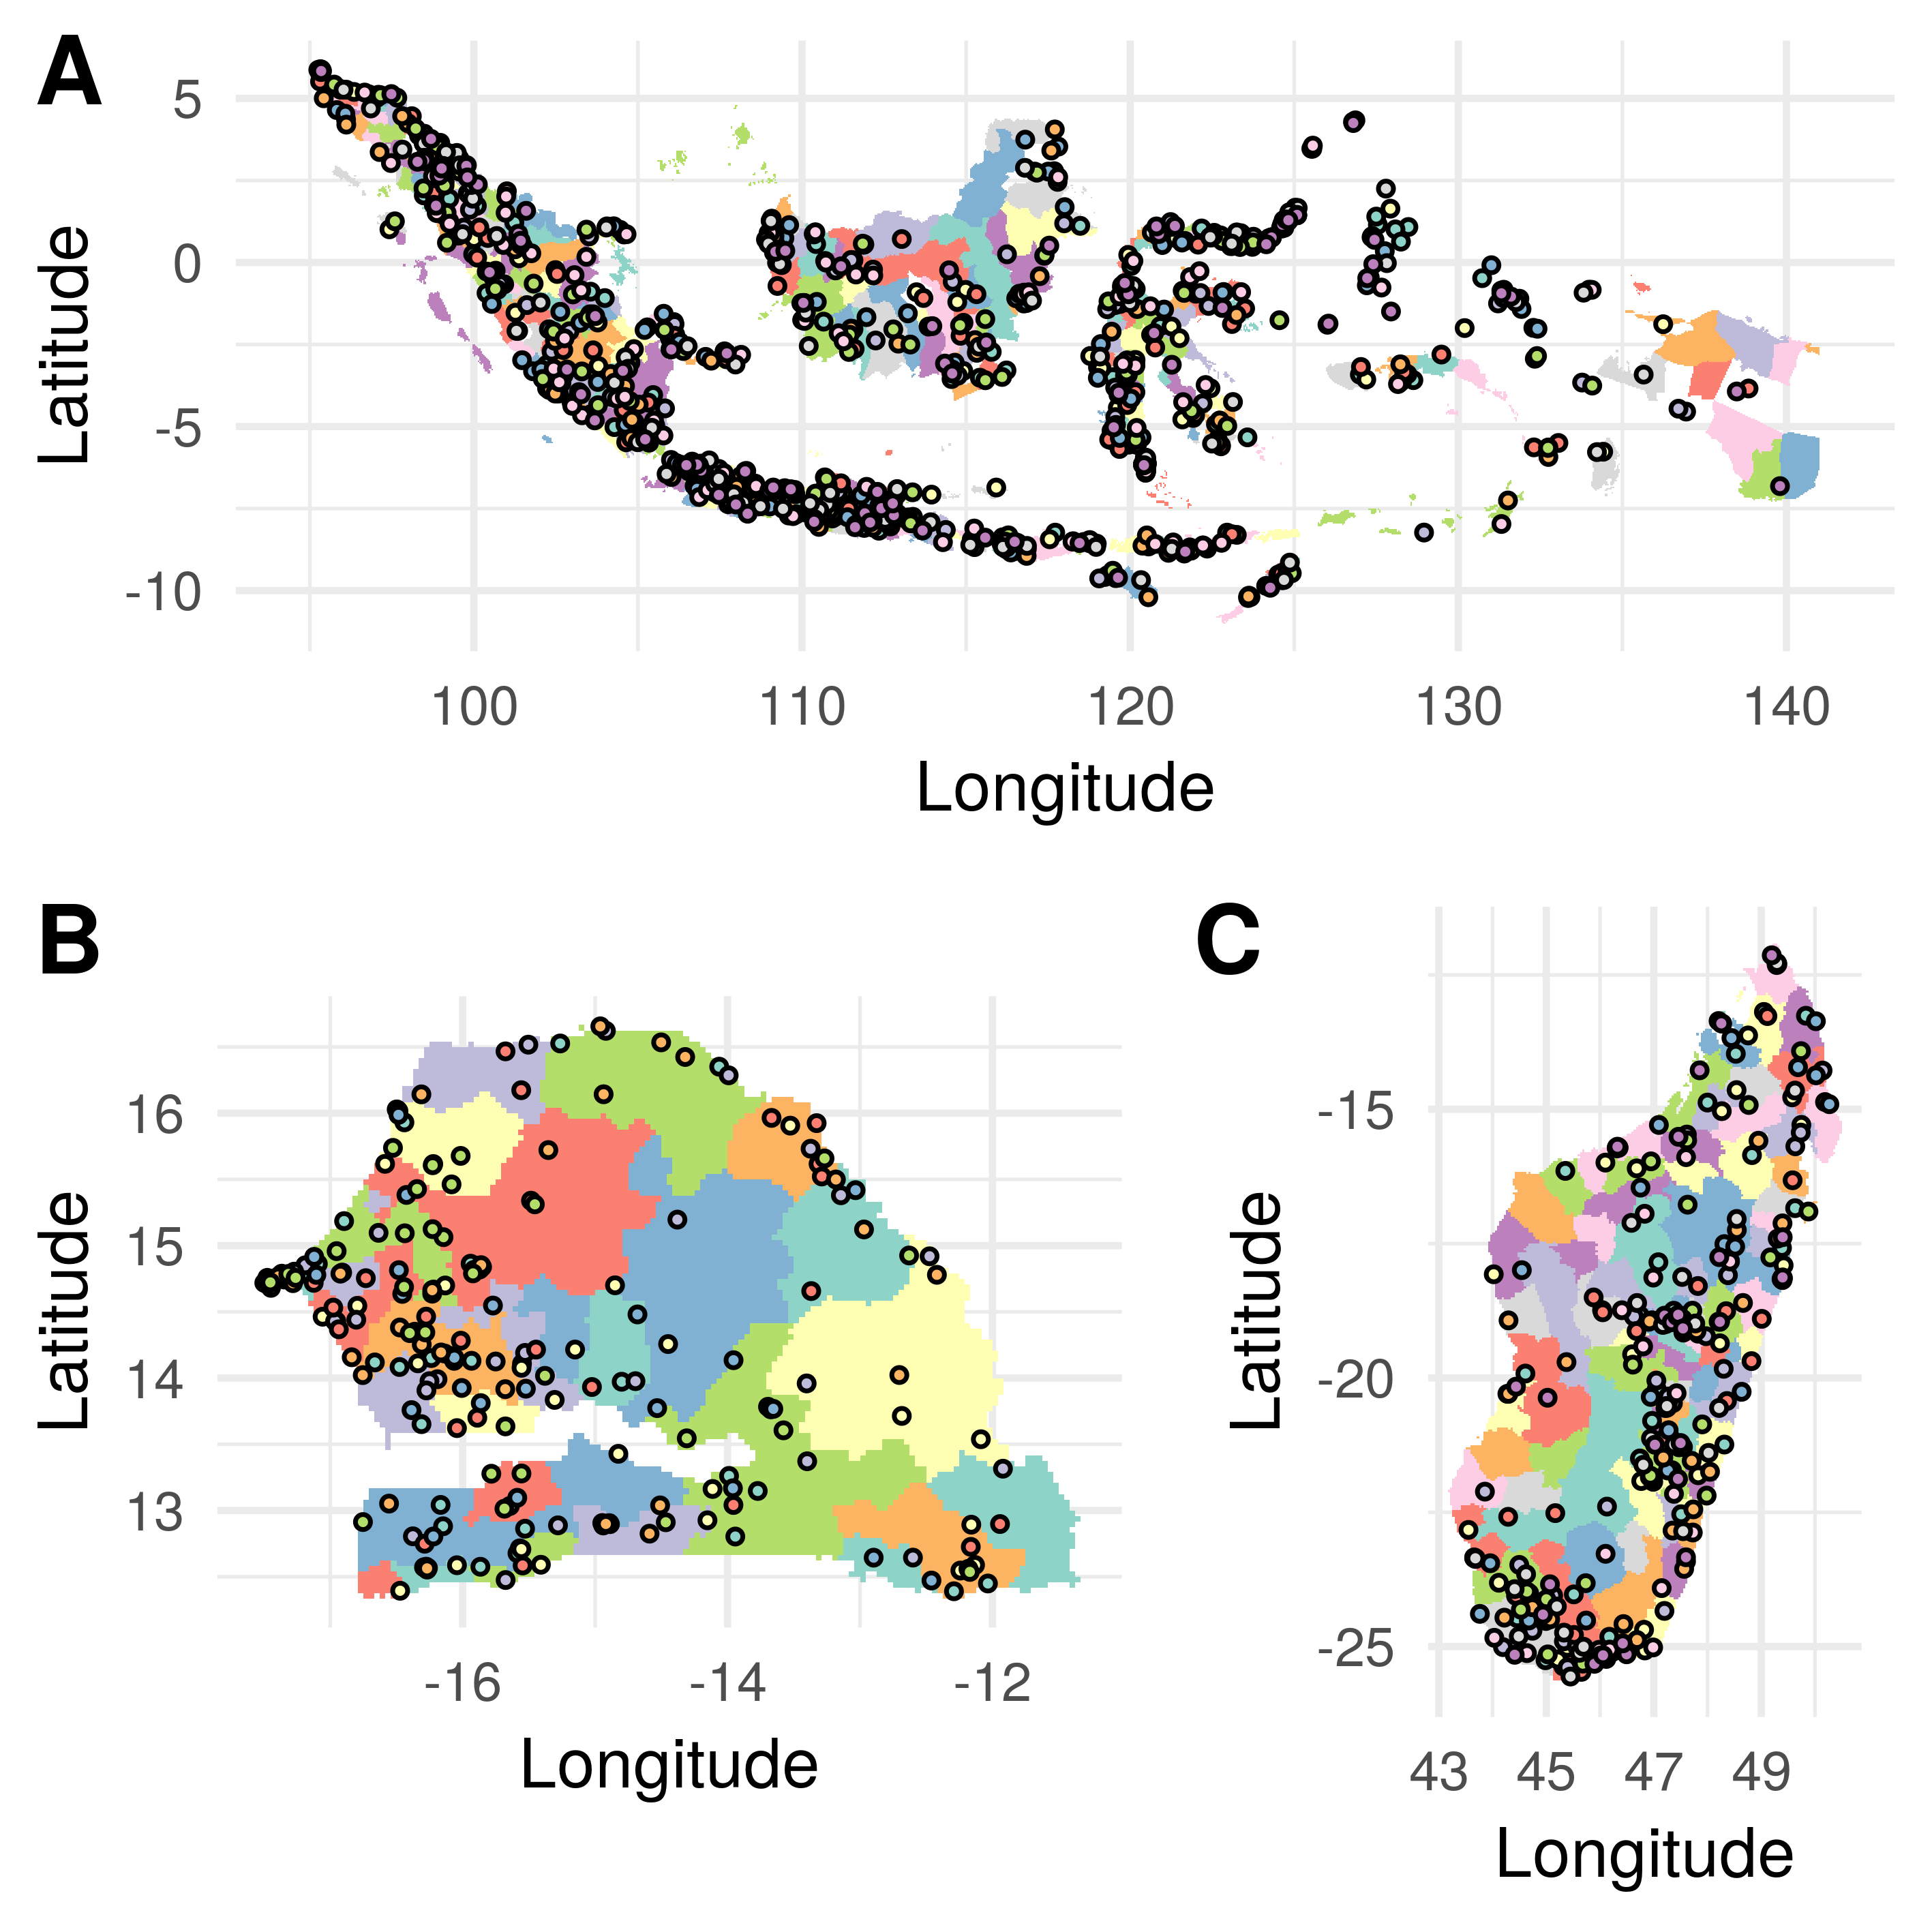
\includegraphics[width = 0.9\textwidth]{figures/random_crossvalidation_full.png} %\caption{Indonesia random crossvalidation} 

\caption{{\bf Random cross-validation scheme for Indonesia, Senegal and Madagascar.} The fold for both aggregated incidence data and prevalence point data is shown.}
\label{fig:cv_random}
\end{figure}


\begin{figure}[!h]
% to be removed before submission
\centering

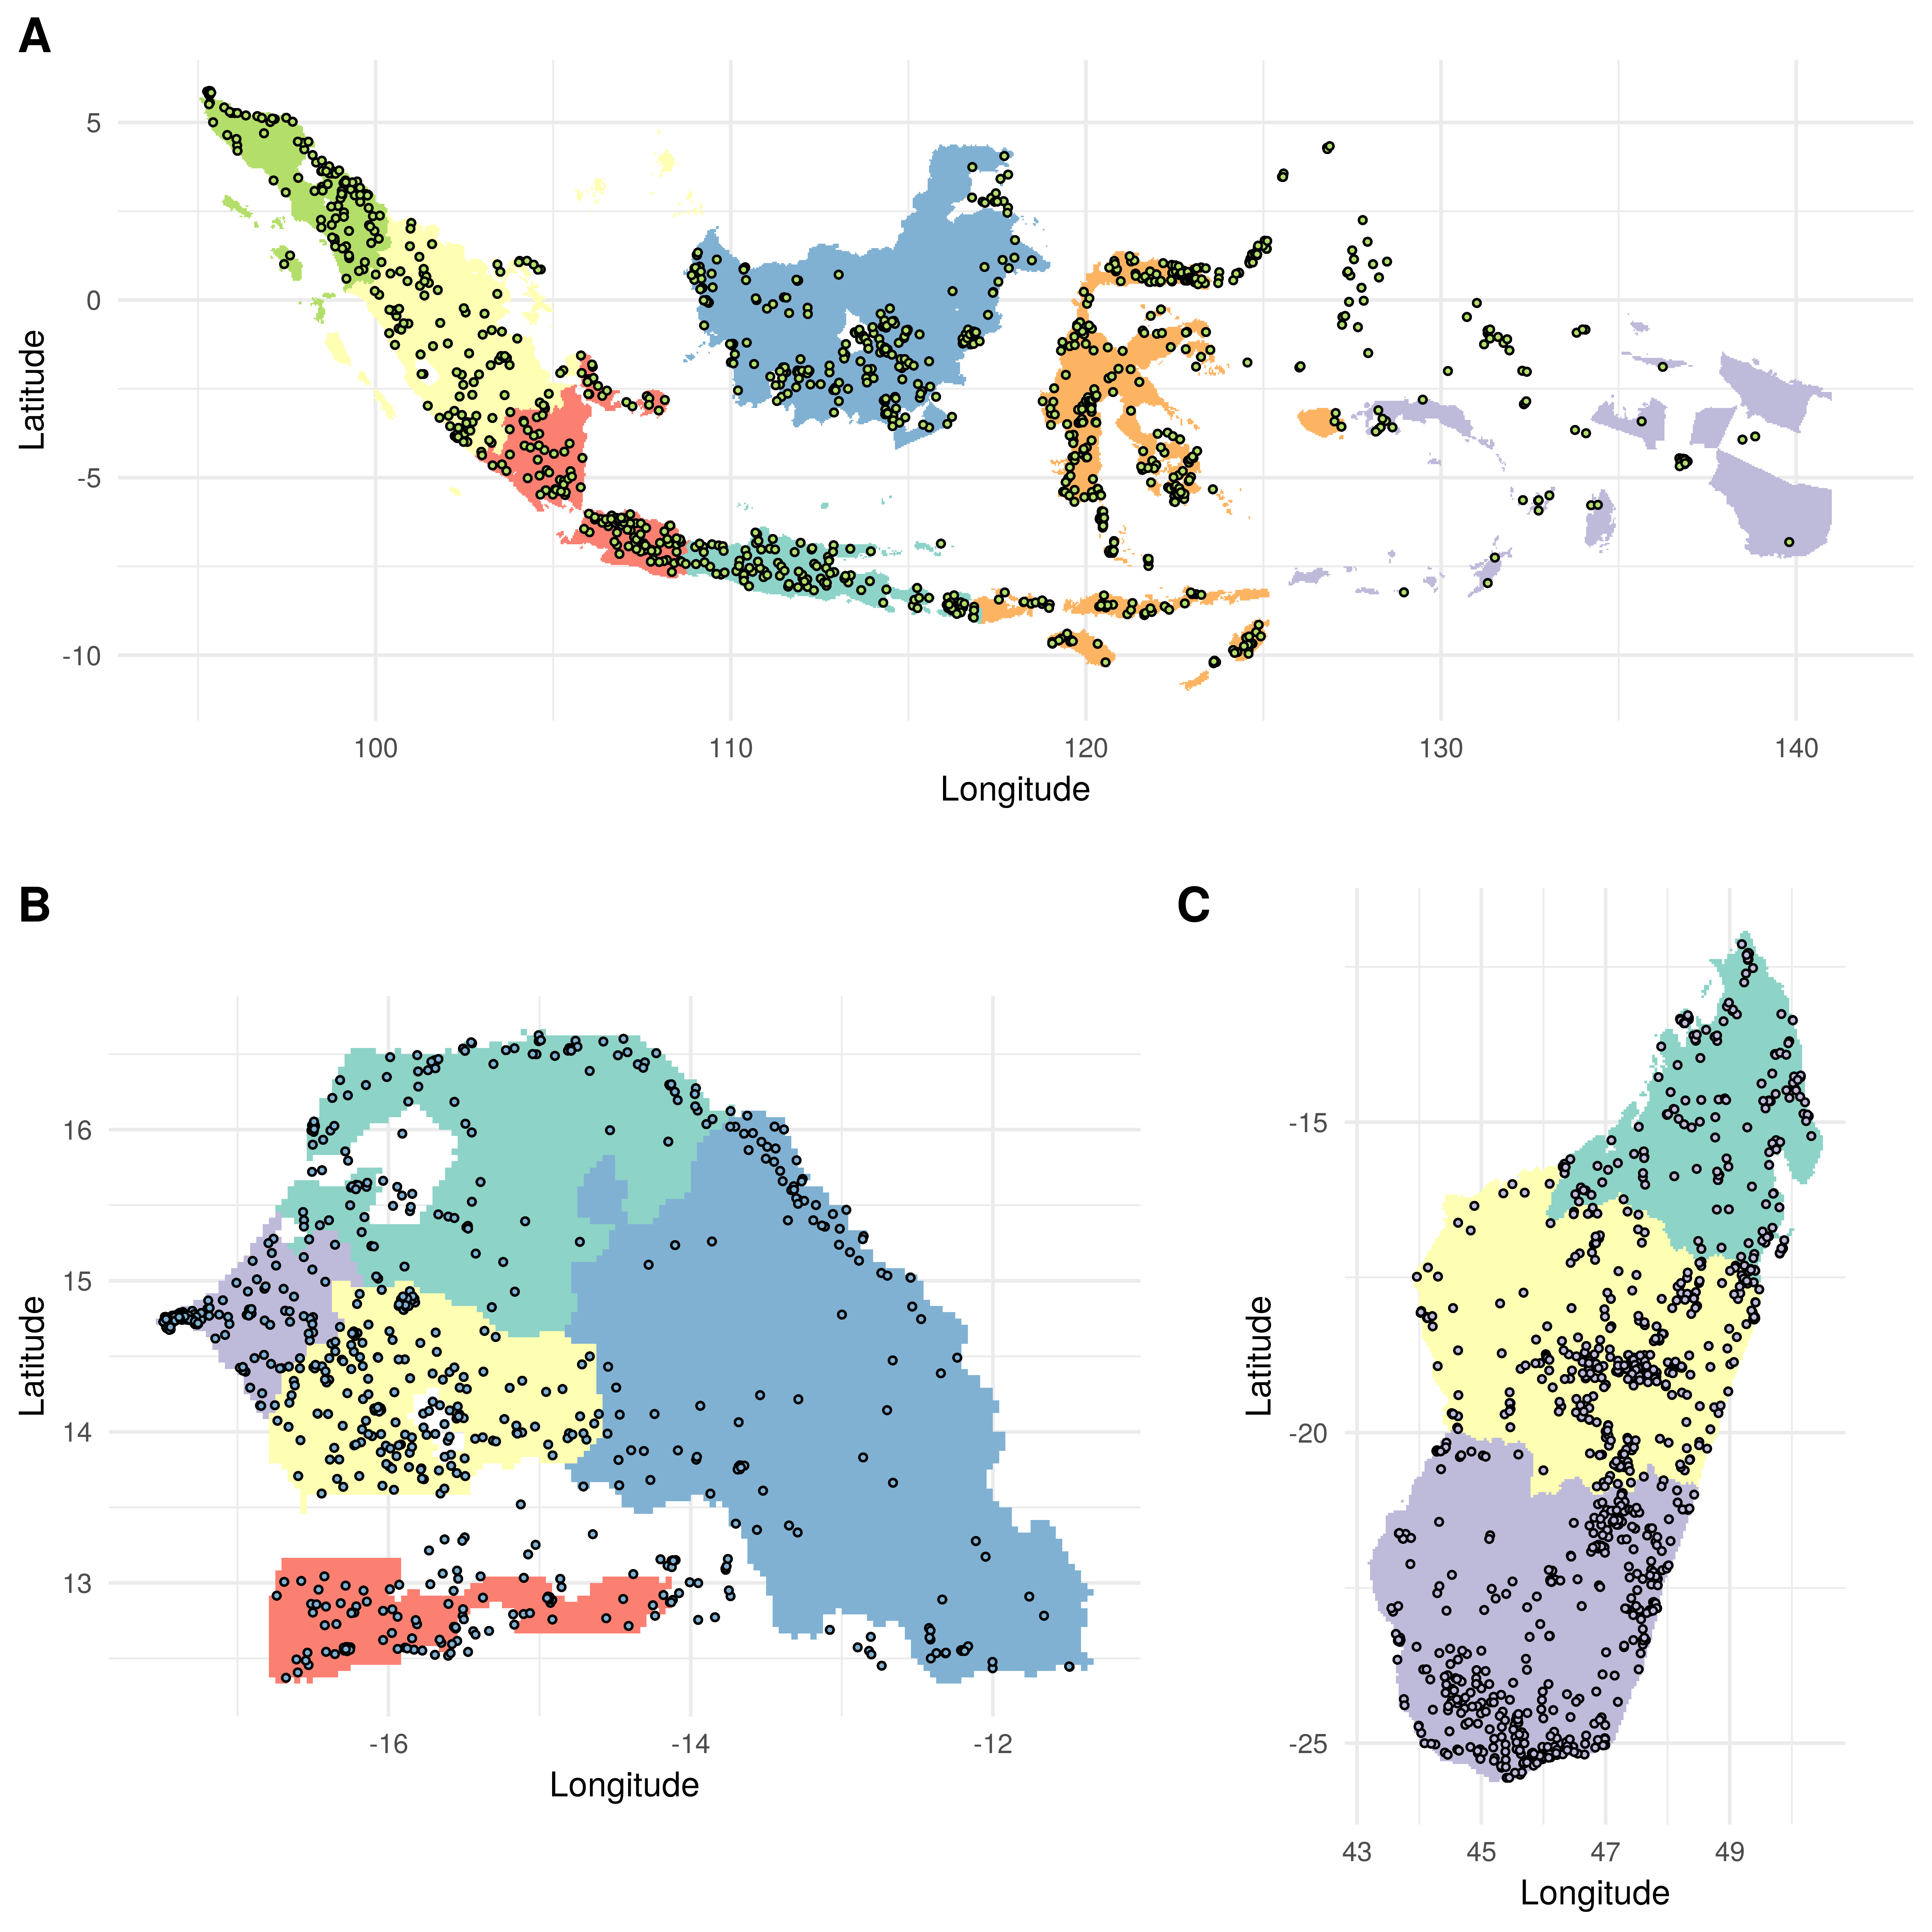
\includegraphics[width = 0.9\textwidth]{figures/spatial_crossvalidation_full.png} %\caption{Indonesia random crossvalidation} 

\caption{{\bf Spatial cross-validation scheme for Indonesia, Senegal and Madagascar.} The fold for both aggregated incidence data and prevalence point data is shown.}
\label{fig:cv_spatial}
\end{figure}



In the second validation scheme the data was split into spatial cross-validation folds (see Figure~\ref{fig:cv_spatial}).
The number of folds was seven for Indonesia, seven for Senegal and three for Madagascar due to their differing size and geographies.
The data was divided by combining the point locations and the centroids of the polygons and performing k means clustering.
This scheme is testing the models' ability to predict into new areas with little information from the spatial random field.

In both cases we examined performance metrics for both the withheld prevalence data and the withheld incidence data.
As there is no good way of combining predictive error from both types of data into one performance metric, we considered performance separately throughout.
Our main performance metric was mean absolute error.
To assess how well the models are calibrated we considered coverage of the 80\% predictive credible intervals on the hold-out data.



% Results and Discussion can be combined.
%%%%%%%%%%%%%%%%%%%%%%%%%%%%%%%%%%%%%%%%%%%%%%%%%%%%%%%%%%%%%%%%%%%%%%%%%%%%%%%%%%%%%%%%%%%%%%%%%%%%%
\section*{Results and Discussion}
%%%%%%%%%%%%%%%%%%%%%%%%%%%%%%%%%%%%%%%%%%%%%%%%%%%%%%%%%%%%%%%%%%%%%%%%%%%%%%%%%%%%%%%%%%%%%%%%%%%%%




%figure 3 and 4. data and predicted incidence maps. Indonesia and Senegal only. Fig 3 ind, fig 4 rand. Data, Rand, Spatial for best model? Joint model?

\begin{figure}[!h]
% to be removed before submission
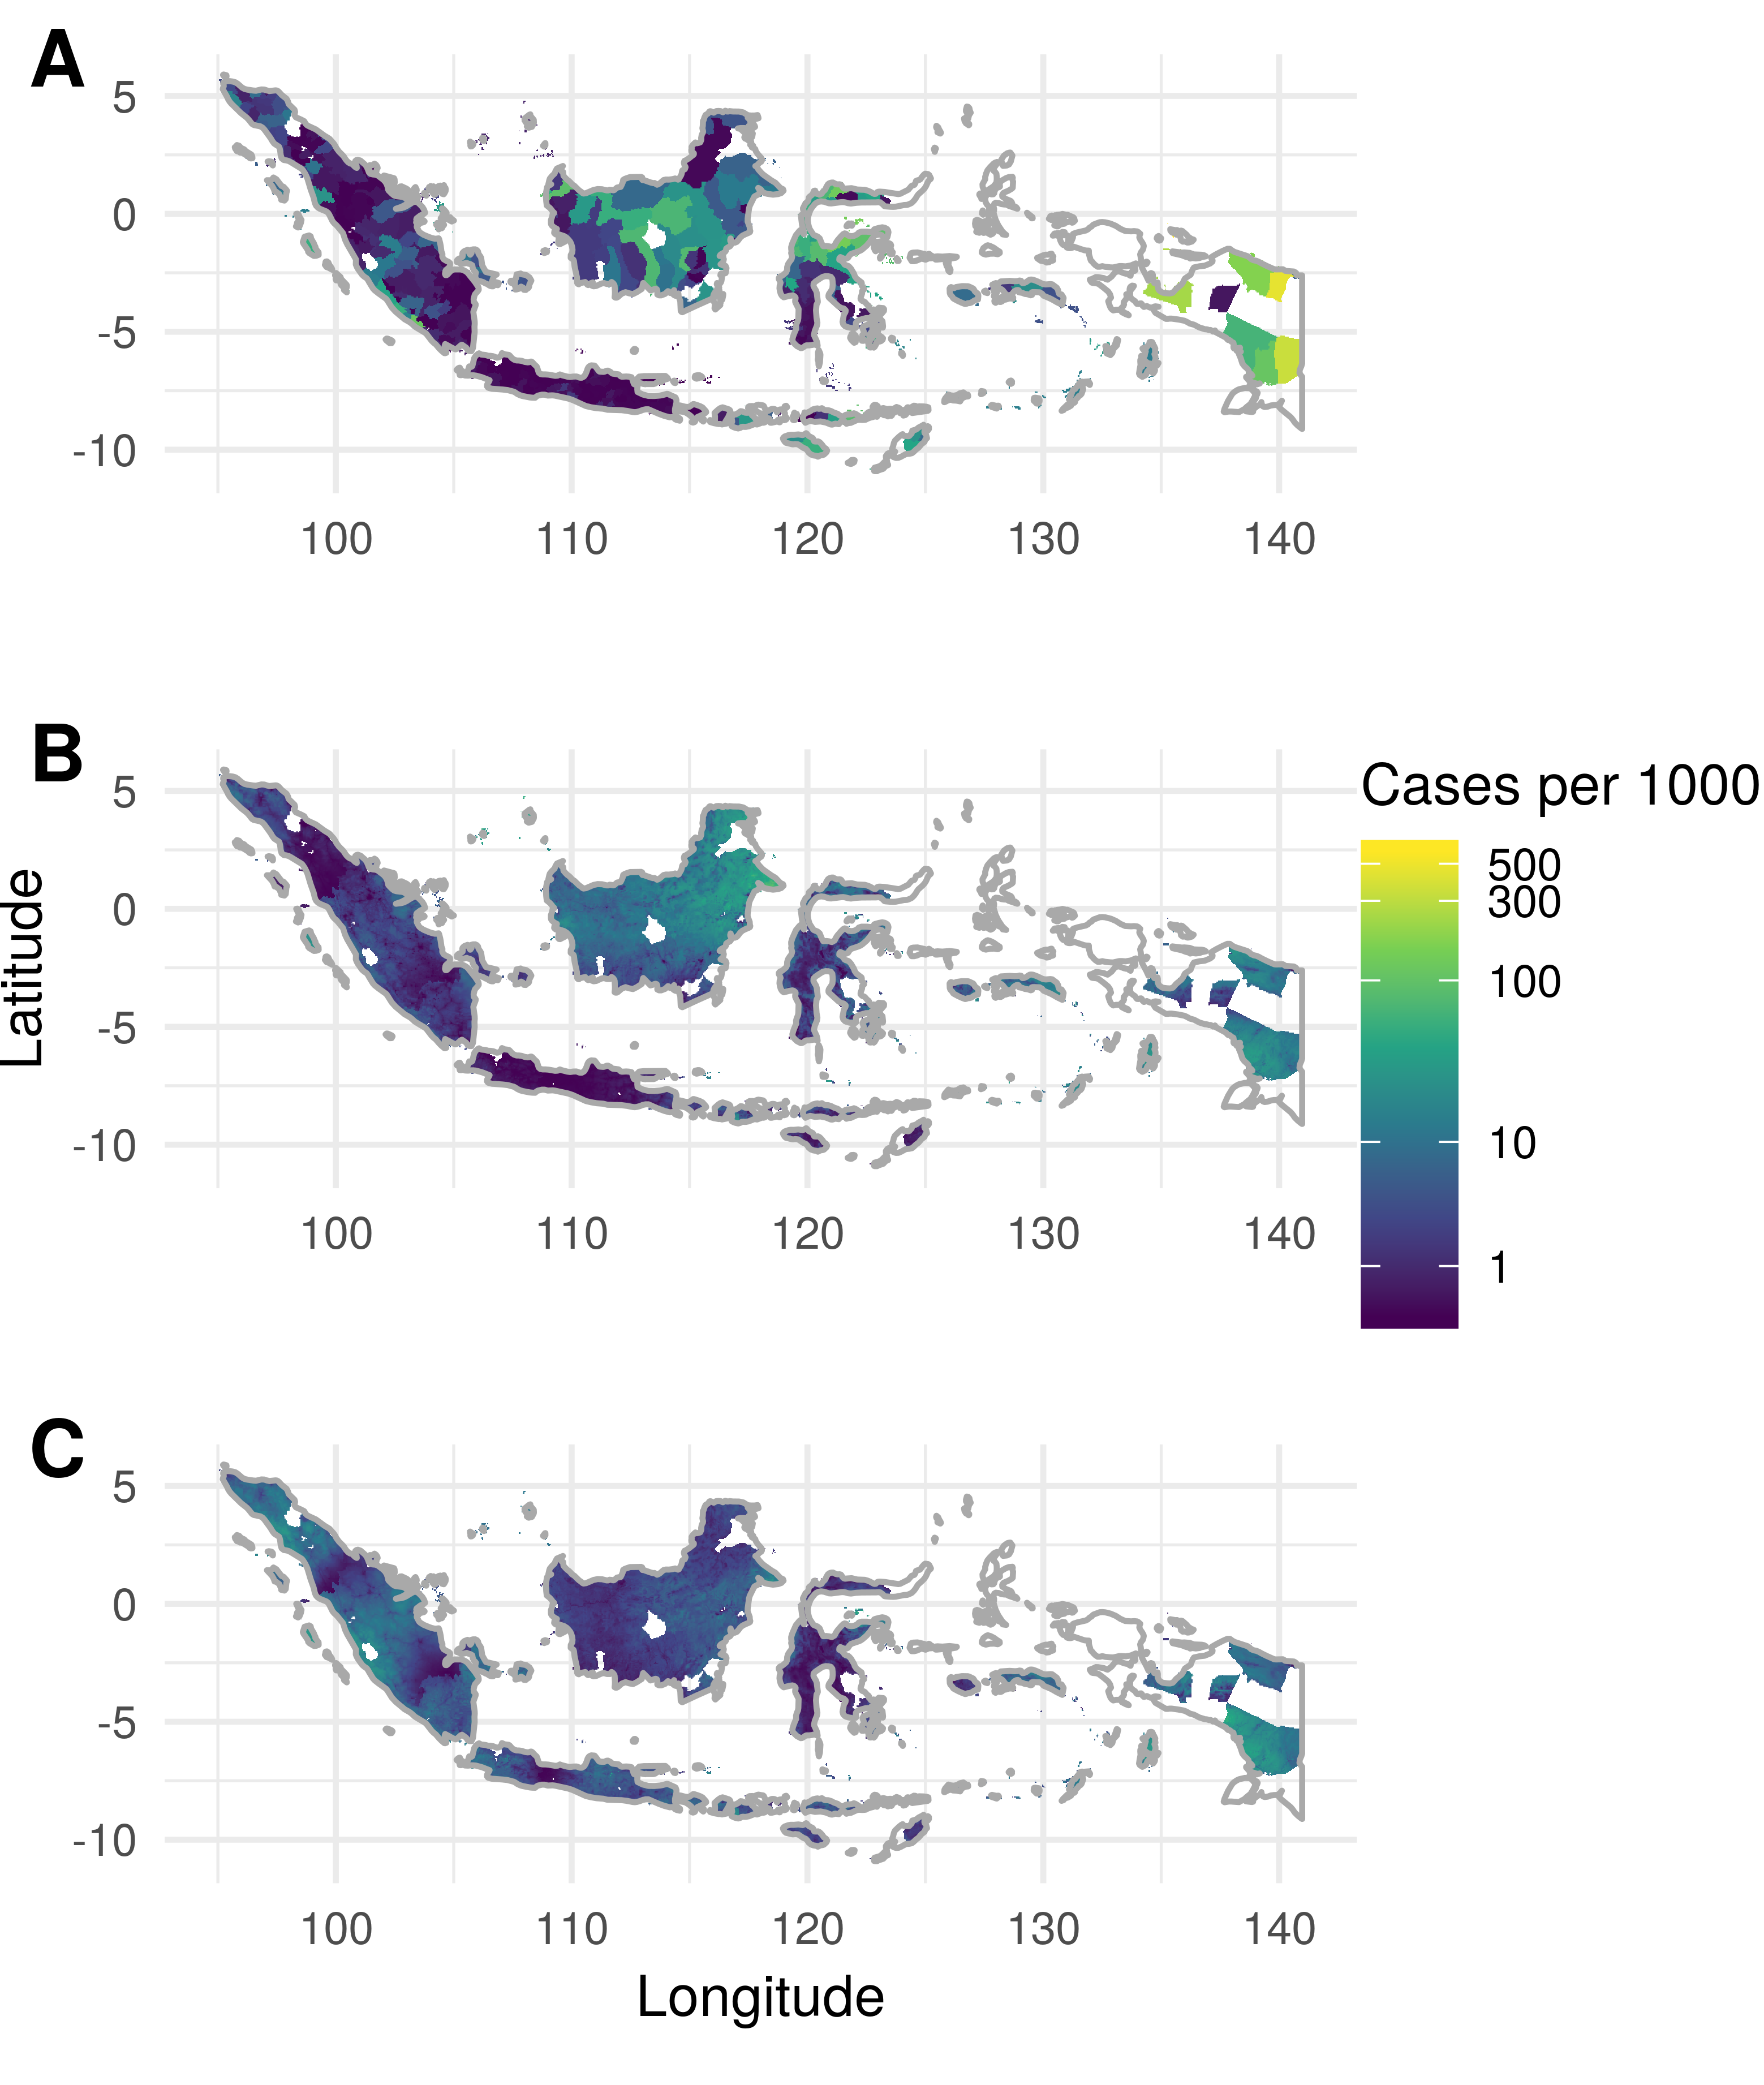
\includegraphics[width = 0.9\textwidth]{figures/idn_both_cv12_preds.png}
\caption{{\bf Input incidence data and predicted incidence maps. } 
The incidence (log10) data (top), predicted log10 incidence from the joint model for randomly sampled out-of-sample polygons (middle) and predicted log10 incidence from the joint model for spatially sampled out-of-sample polygons (bottom) for Indonesia.
}
\label{predobsmapidn}
\end{figure}




\begin{figure}[!h]
% to be removed before submission
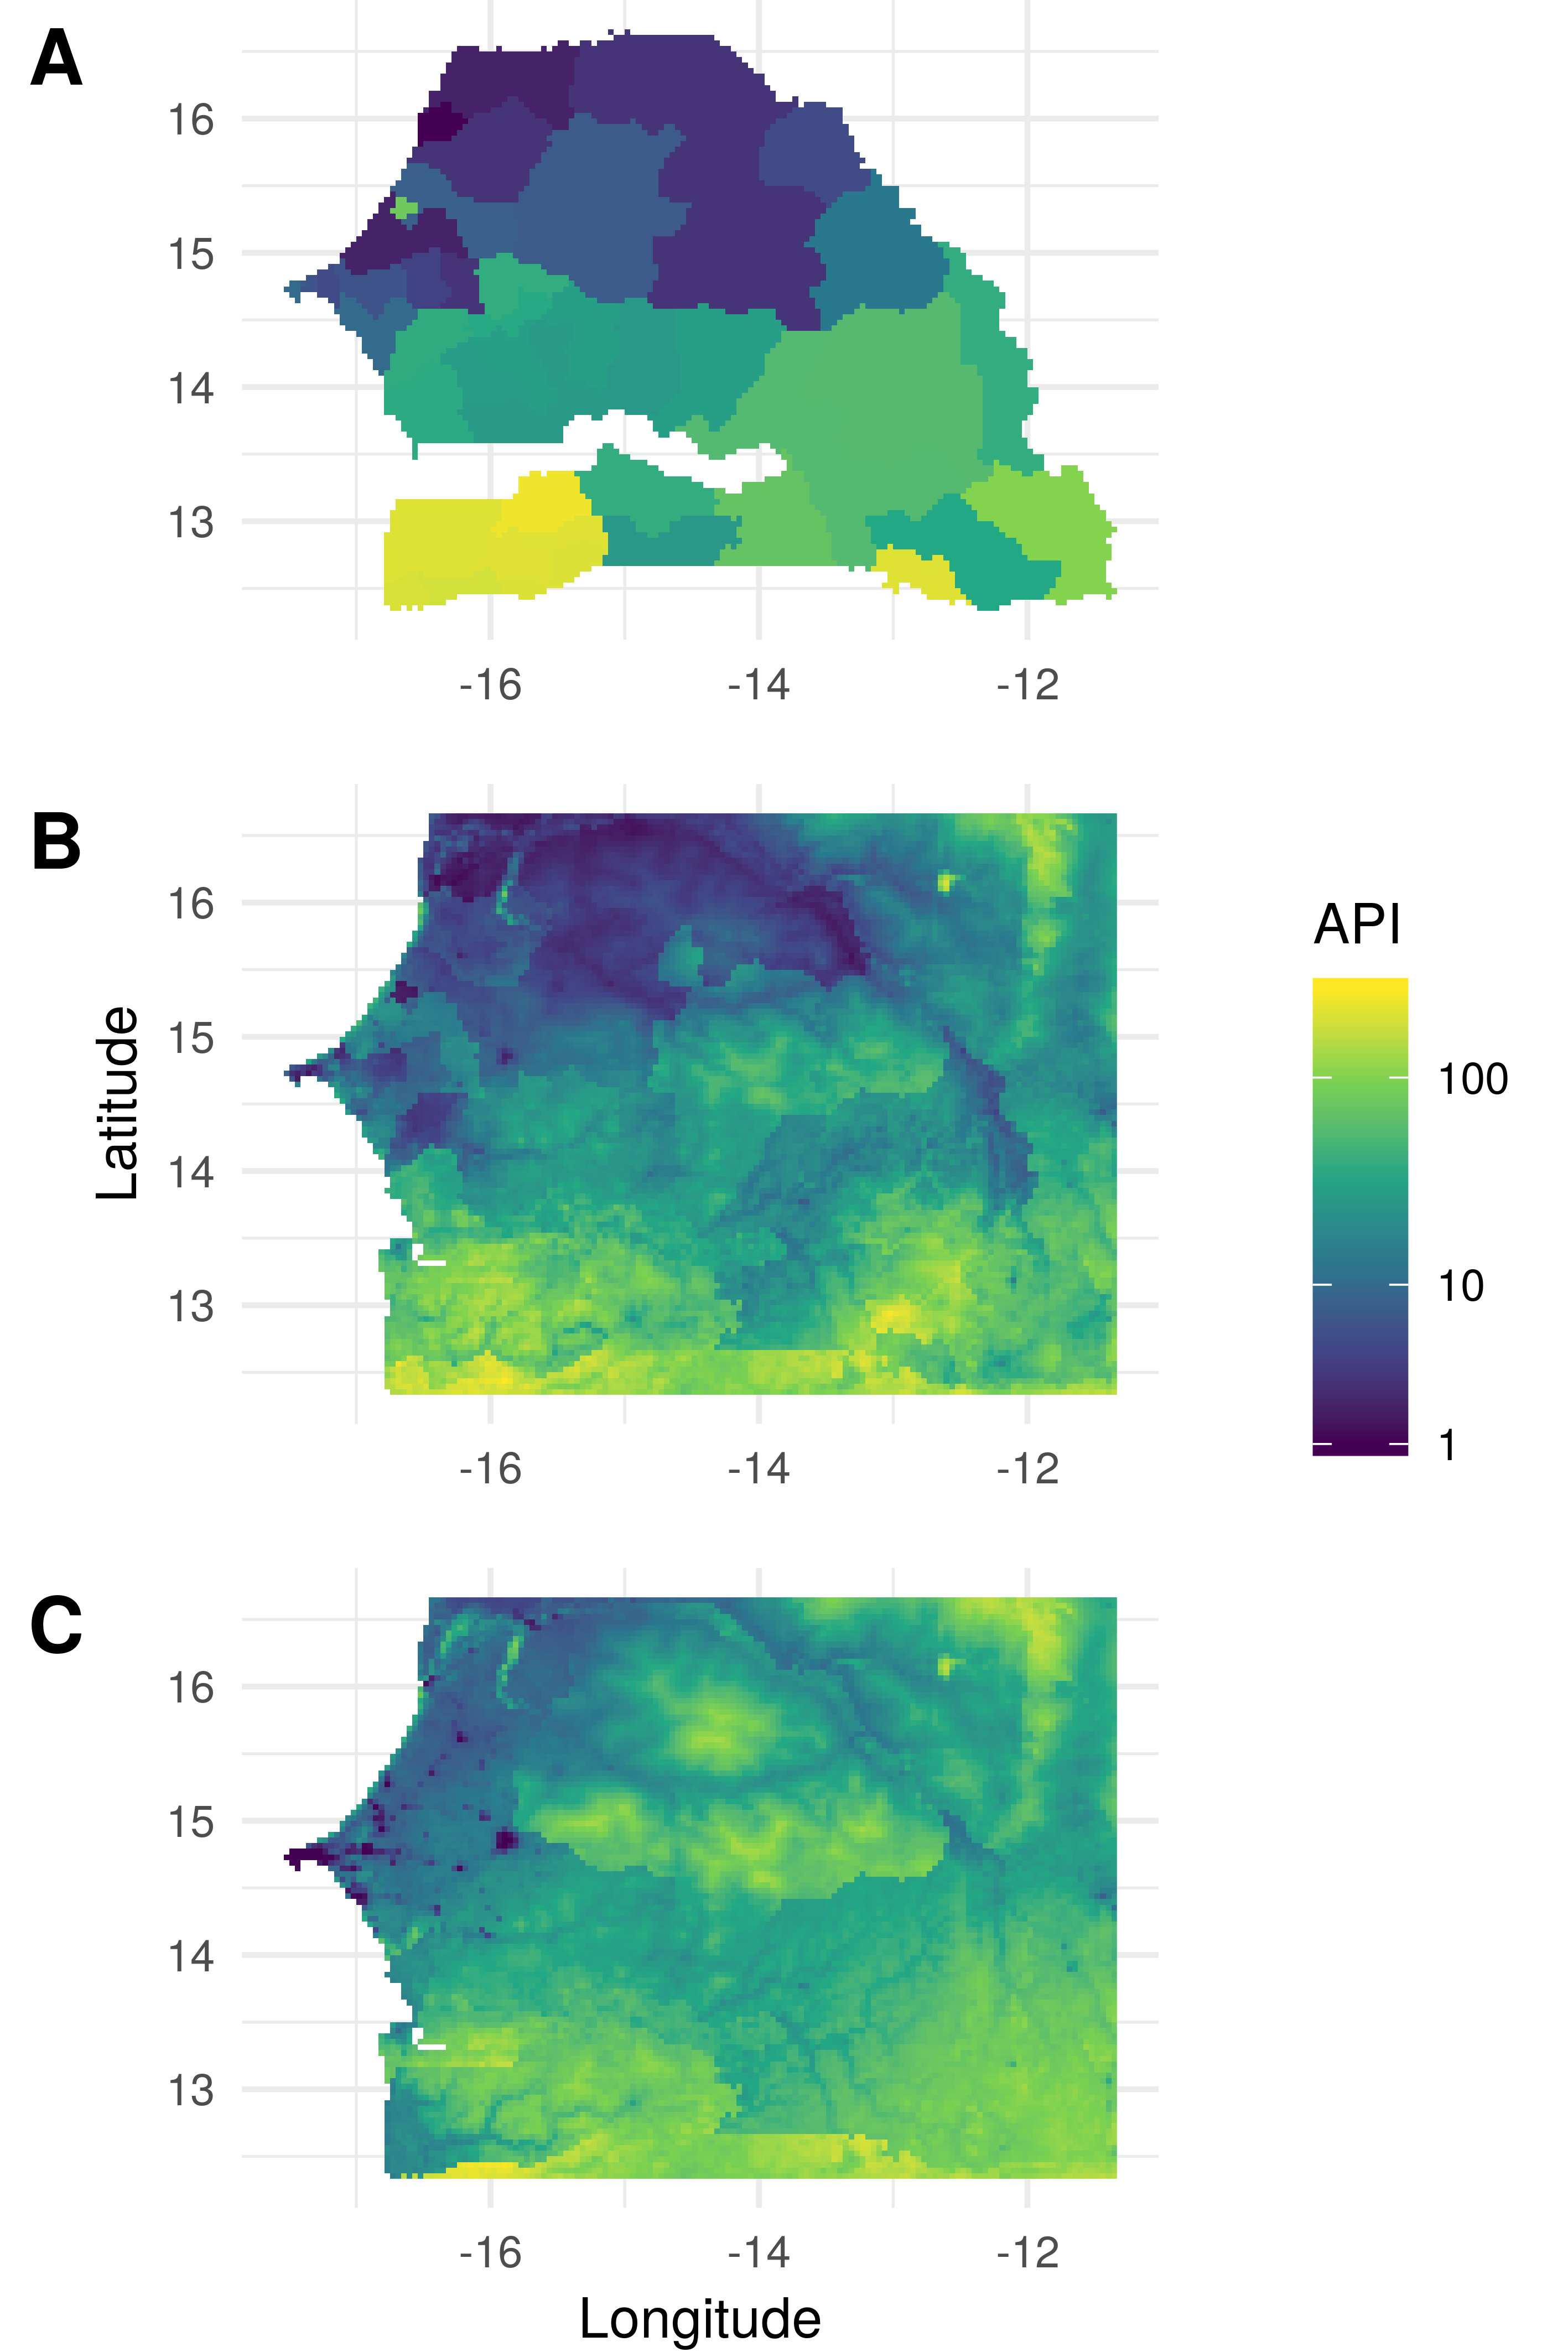
\includegraphics[width = 0.9\textwidth]{figures/sen_both_cv12_preds.png}
\caption{{\bf Input incidence data and predicted incidence maps. } 
The incidence (log10) data, predicted log10 incidence from the joint model for randomly sampled out-of-sample polygons (middle) and predicted log10 incidence from the joint model for spatially sampled out-of-sample polygons (bottom) for Senegal.
}
\label{predobsmapsen}
\end{figure}



\begin{table}[!ht]
\begin{adjustwidth}{-2.25in}{0in} % Comment out/remove adjustwidth environment if table fits in text column.
\centering
\caption{
{\bf Summary of out-of-sample accuracy for random crossvalidation experiment.}}
\begin{tabular}{llllll}
\hline
{\bf Holdout data} & {\bf Country} &  {\bf Points} & {\bf Polygons} & {\bf Joint} \\
\thickhline 
Incidence & Indonesia & 18.33 & 14.02 &  14.09\\
& Senegal & 51.24 & 26.74 &  28.45\\
& Madagascar & 85.54 & 37.45 &  34.49\vspace{3mm}\\
Prevalence & Indonesia & 0.010 & 0.010 &  0.010\\
& Senegal & 0.015 & 0.024 &  0.024\\
& Madagascar & 0.054 & 0.059 &  0.059\\
\end{tabular}
\begin{flushleft}
Mean absolute error of predicted incidence rate and weighted mean absolute error of prevalence against out-of-sample observed data for three countries.
The data were split randomly into 10 groups stratified by data type (incidence polygon and prevalence points).
\end{flushleft}
\label{table1}
\end{adjustwidth}
\end{table}


\begin{table}[!ht]
\begin{adjustwidth}{-2.25in}{0in} % Comment out/remove adjustwidth environment if table fits in text column.
\centering
\caption{
{\bf Summary of out-of-sample accuracy for spatial crossvalidation experiment.}}
\begin{tabular}{llllll}
\hline
{\bf Holdout data} & {\bf Country} &  {\bf Points} & {\bf Polygons} & {\bf Joint} \\
\thickhline 
Incidence & Indonesia &  18.13 &  14.77 &   15.02\\
& Senegal &  51.17 &  41.43 &   36.76\\
& Madagascar & 107.32 &  71.44 &   65.50\vspace{3mm}\\
Prevalence & Indonesia & 0.011 & 0.010 &  0.010\\
& Senegal & 0.015 & 0.019 &  0.019\\
& Madagascar & 0.069 & 0.066 &  0.065\\
\end{tabular}
\begin{flushleft}
Mean absolute error of predicted incidence rate and weighted mean absolute error of prevalence against out-of-sample observed data for three countries.
The data were split spatiall into 5 groups.
\end{flushleft}
\label{table2}
\end{adjustwidth}
\end{table}




%figure 5, 6. Spat and random cv. PR vs Poly columns, countries as rows, model as colour?
\begin{figure}[!h]
% to be removed before submission
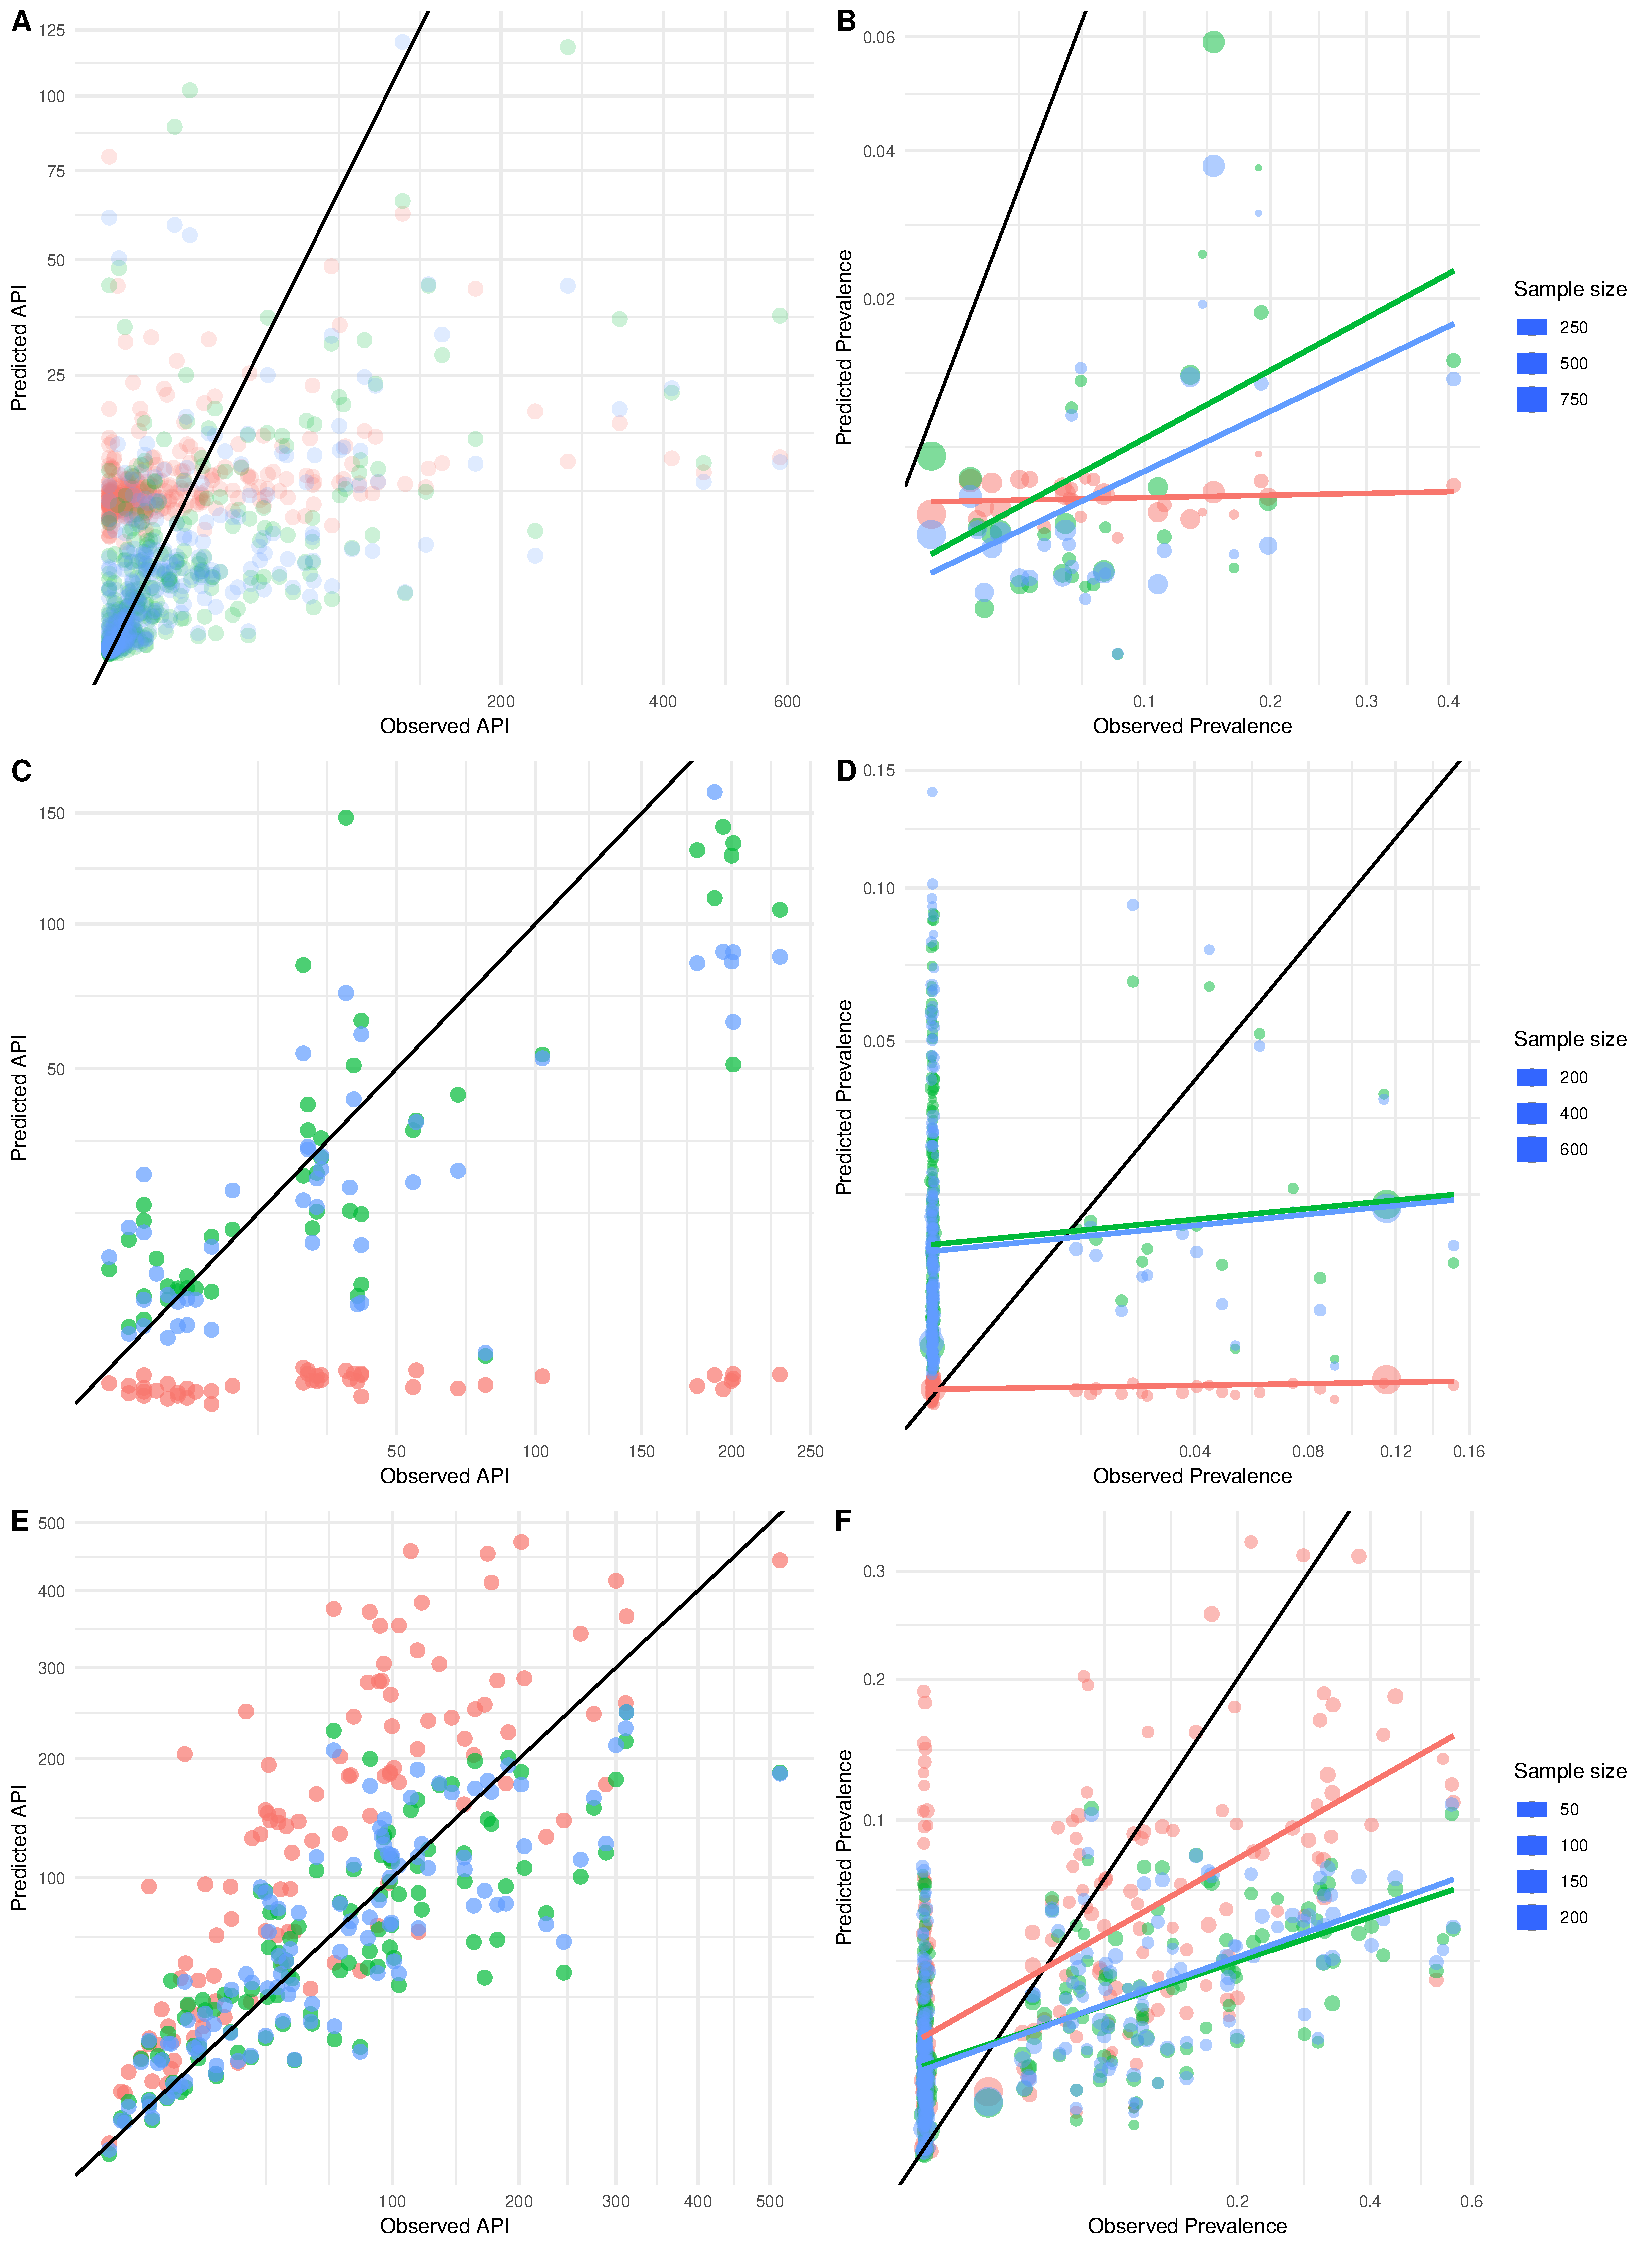
\includegraphics[width = 0.9\textwidth]{figures/random_cv_scatter.pdf} %\caption{Indonesia spatial crossvalidation} 
\caption{{\bf Observed-predicted plots for random cross-validation experiments.}
A-B) Indonesia, C-D) Senegal, E-F) Madagascar. A, C, E) square root aggregated incidence (per 1,000), B, D, F) square root prevalence.
Results from all three models are included with the points only model being shown in orange, the downscaling model being shown in blue and the combined model being shown in green.
}
\label{predobsscatter}
\end{figure}





%figure 5, 6. Spat and random cv. PR vs Poly columns, countries as rows, model as colour?
\begin{figure}[!h]
% to be removed before submission
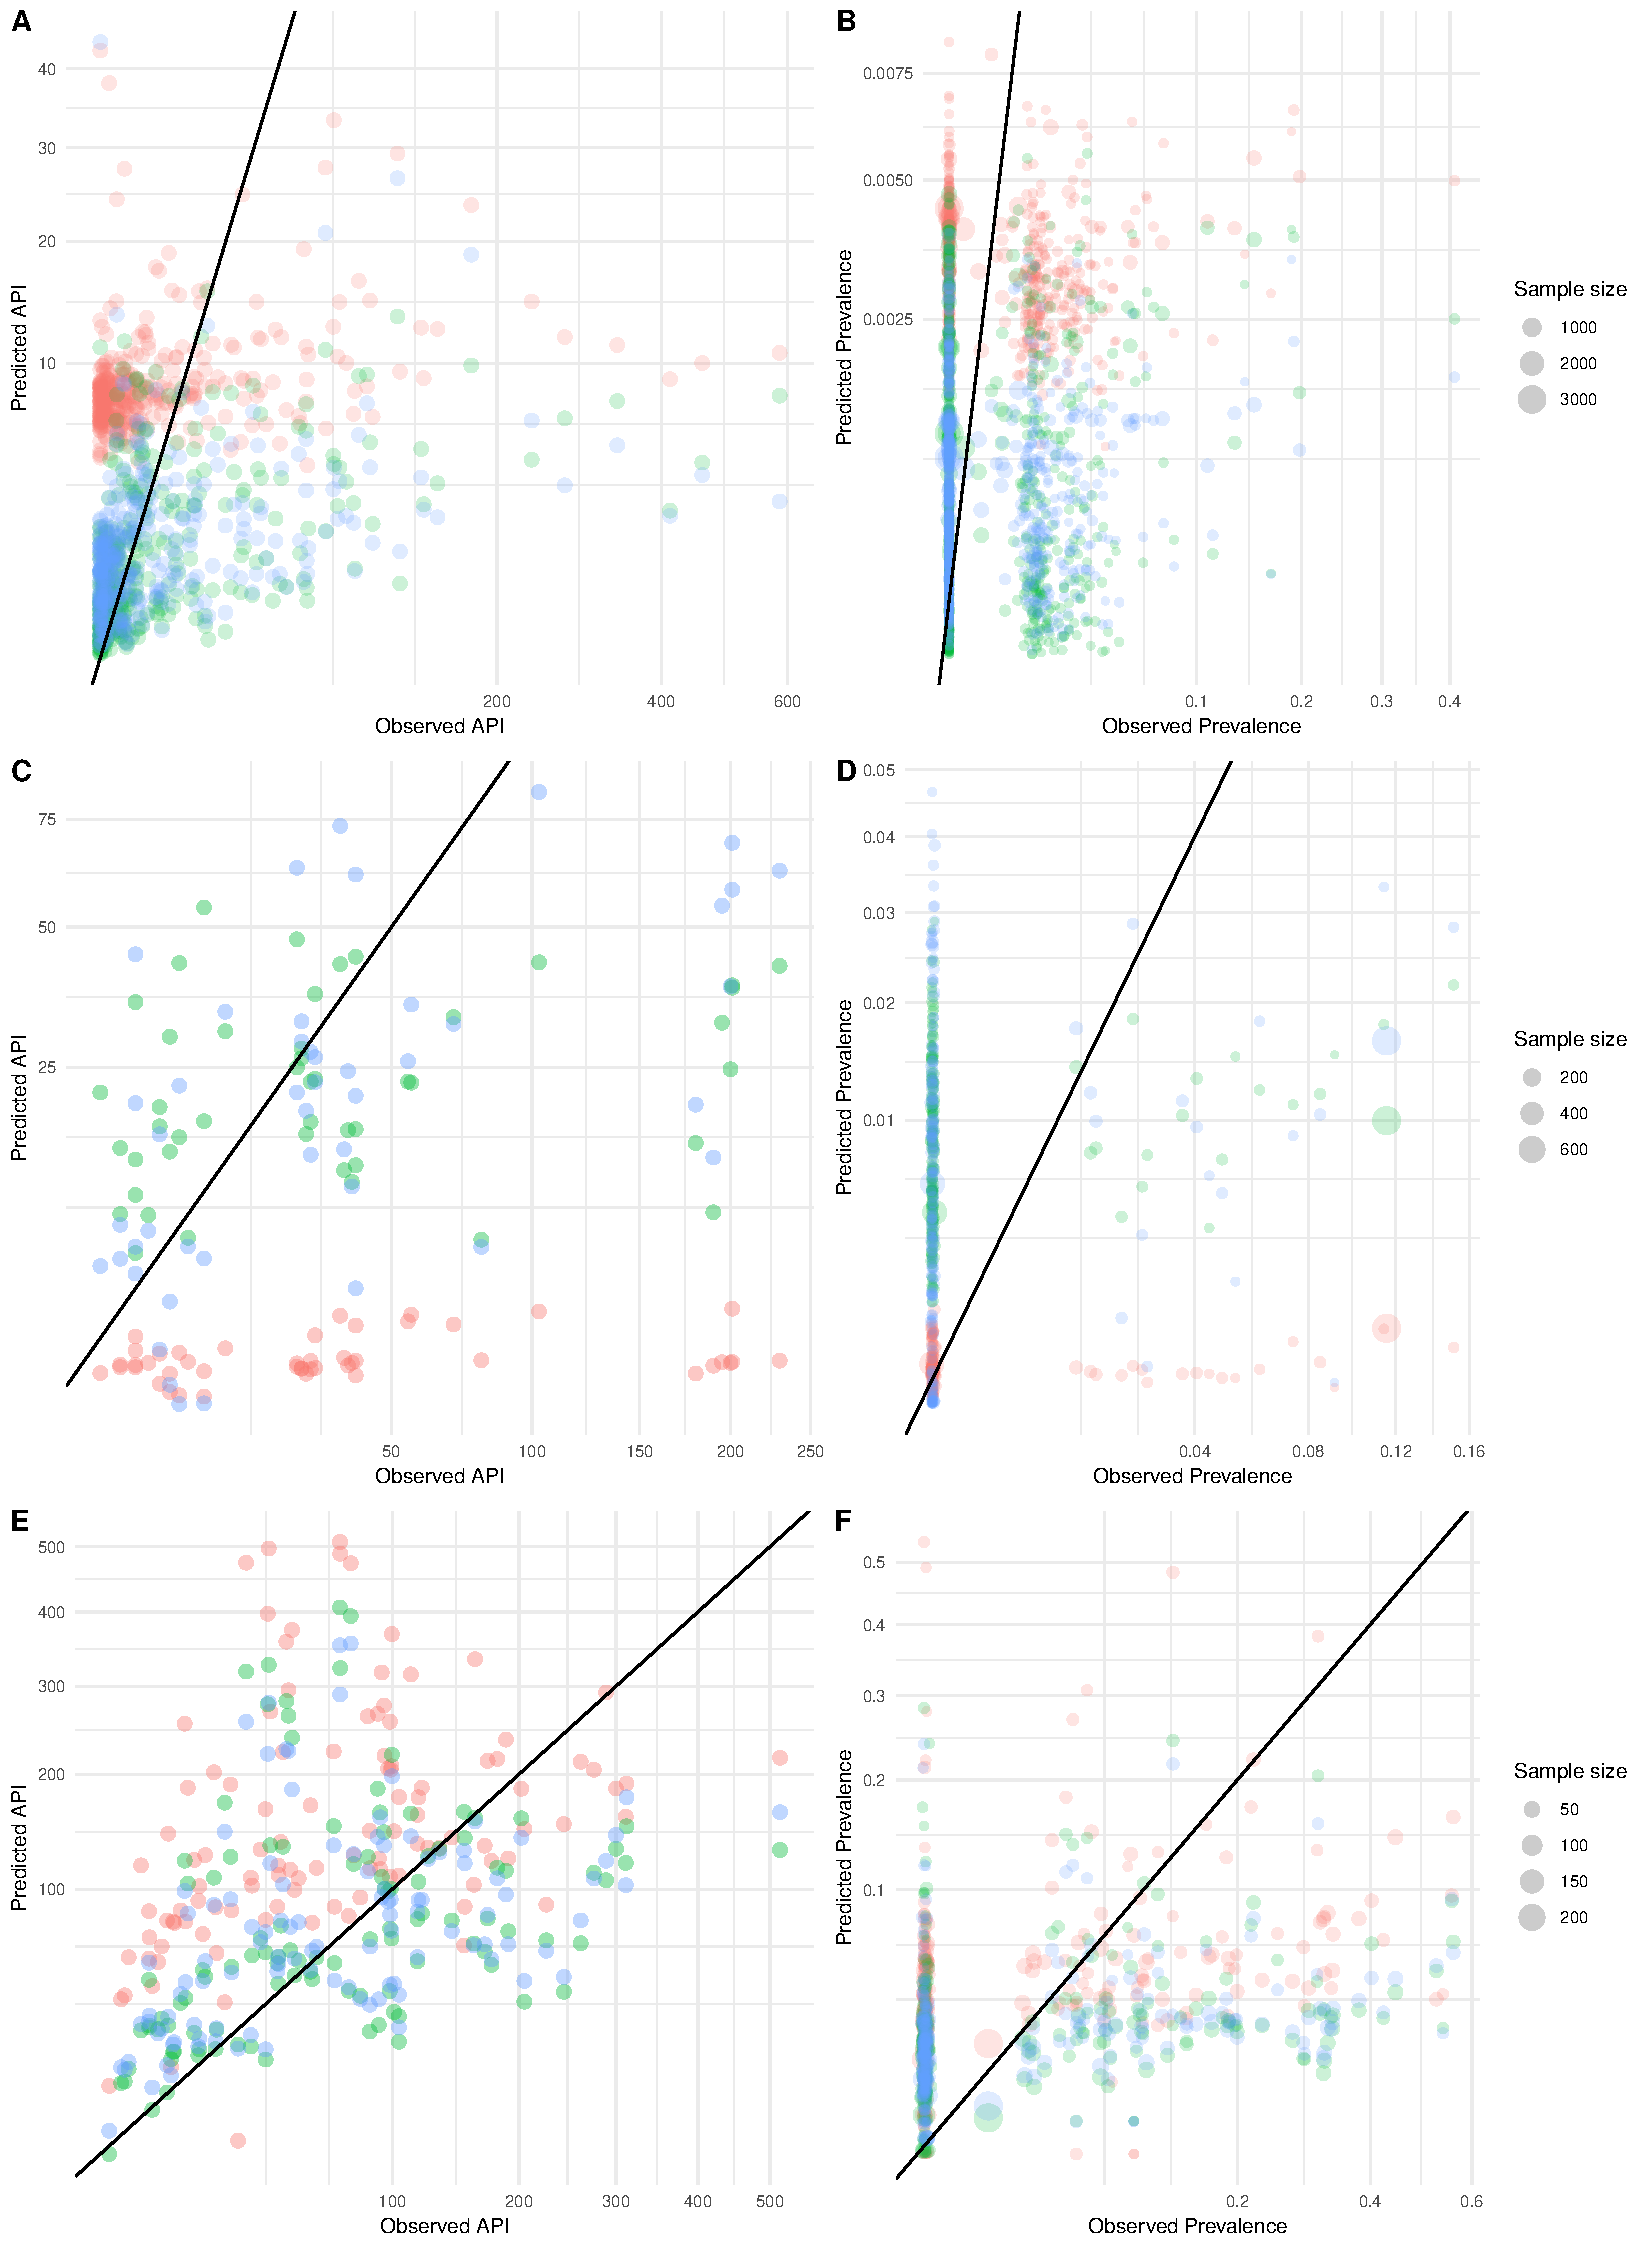
\includegraphics[width = 0.9\textwidth]{figures/spatial_cv_scatter.pdf} %\caption{Indonesia spatial crossvalidation} 
\caption{{\bf Observed-predicted plots for spatial cross-validation experiments.}
A-B) Indonesia, C-D) Senegal, E-F) Madagascar. A, C, E) square root aggregated incidence (per 1,000), B, D, F) square root prevalence.
Results from all three models are included with the points only model being shown in orange, the downscaling model being shown in blue and the combined model being shown in green.
}
\label{predobsscatter}
\end{figure}






\begin{table}[!ht]
\begin{adjustwidth}{-2.25in}{0in} % Comment out/remove adjustwidth environment if table fits in text column.
\centering
\caption{
{\bf Summary of coverage of 80\% credible intervals for.}}
\begin{tabular}{llllll}
\hline
{\bf Holdout data} & {\bf crossvalidation} & {\bf Country} &  {\bf Points} & {\bf Polygons} & {\bf Joint} \\
\thickhline 
Incidence & Random & Indonesia & 0.13 & 0.72 &  0.73\\
&& Senegal & 0.11 & 0.80 &  0.85\\
&& Madagascar & 0.59 & 0.82 &  0.77\vspace{1mm}\\
& Spatial & Indonesia & 0.14 & 0.76 &  0.68\\
&& Senegal & 0.30 & 0.67 &  0.70\\
&& Madagascar & 0.68 & 0.65 &  0.68\vspace{3mm} \\
Prevalence & Random & Indonesia & 0.90 & 0.50 &  0.80\\
&& Senegal & 0.80 & 0.71 &  0.91\\
&& Madagascar & 0.83 & 0.53 &  0.74\vspace{1mm}\\
& Spatial & Indonesia & 0.87 & 0.62 &  0.96\\
&& Senegal & 0.90 & 0.88 &  0.79\\
&& Madagascar & 0.93 & 0.68 &  0.83\\
\end{tabular}
\begin{flushleft}

\end{flushleft}
\label{table3}
\end{adjustwidth}
\end{table}

%%%%%%%%%%%%%%%%%%%%%%%%%%%%%%%%%%%%%%%%%%%%%%%%%%%%%%%%%%%%%%%%%%%%%%%%%%%%%%%%%%%%%%%%%%%%%%%%%%%%%
\section*{Conclusion}
%%%%%%%%%%%%%%%%%%%%%%%%%%%%%%%%%%%%%%%%%%%%%%%%%%%%%%%%%%%%%%%%%%%%%%%%%%%%%%%%%%%%%%%%%%%%%%%%%%%%%





\section*{Supporting information}

% Include only the SI item label in the paragraph heading. Use the \nameref{label} command to cite SI items in the text.
\paragraph*{S1 Fig.}
\label{S1_Fig}
{\bf Bold the title sentence.} Add descriptive text after the title of the item (optional).


\section*{Acknowledgments}
Thanks everyone.
\nolinenumbers

% Either type in your references using
% \begin{thebibliography}{}
% \bibitem{}
% Text
% \end{thebibliography}
%
% or
%
% Compile your BiBTeX database using our plos2015.bst
% style file and paste the contents of your .bbl file
% here. See http://journals.plos.org/plosone/s/latex for 
% step-by-step instructions.
% 
\bibliography{Malaria} 

%\begin{thebibliography}{10}


%\end{thebibliography}



\end{document}

